\documentclass[11pt,a4paper]{article}

\usepackage[a4paper,margin=2.3cm]{geometry}
\usepackage{amsmath,amssymb,bm,mathtools}
\usepackage{booktabs,array,longtable}
\usepackage{graphicx}
\usepackage{xcolor}
\usepackage{listings}
\usepackage{microtype}
\usepackage{hyperref}
\usepackage[capitalise,noabbrev]{cleveref}

\hypersetup{
  colorlinks=true,
  linkcolor=blue!55!black,
  citecolor=green!35!black,
  urlcolor=blue!60!black,
  pdftitle={Symmetry-Aware Raman and Infrared Spectroscopy in TD-SCHA}
}

\definecolor{codeblue}{RGB}{34,82,126}
\definecolor{codegray}{RGB}{245,246,247}
\lstset{
  basicstyle=\ttfamily\small,
  keywordstyle=\color{codeblue}\bfseries,
  commentstyle=\color{green!35!black},
  backgroundcolor=\color{codegray},
  frame=single,
  framesep=5pt,
  showstringspaces=false,
  breaklines=true,
  columns=fullflexible,
  language=Python
}

\newcommand{\dd}{\mathrm{d}}
\newcommand{\ii}{\mathrm{i}}
\newcommand{\Tr}{\operatorname{Tr}}
\newcommand{\Span}{\operatorname{span}}
\newcommand{\Oh}{\mathrm{O_h}}
\newcommand{\epsinf}{\bm\varepsilon_\infty}
\newcommand{\angstrom}{\text{\AA}}
% Generated by benchmark_spectroscopy.py; do not edit.
\newcommand{\BenchSteps}{256}
\newcommand{\RamanRequested}{7}
\newcommand{\RamanNonzero}{3}
\newcommand{\RamanIndependent}{1}
\newcommand{\RamanError}{3.04e-14}
\newcommand{\RamanLegacyTime}{14.645}
\newcommand{\RamanNewTime}{1.482}
\newcommand{\RamanSpeedup}{9.88}
\newcommand{\IRIndependent}{1}
\newcommand{\IRError}{3.05e-14}
\newcommand{\IRLegacyTime}{14.580}
\newcommand{\IRNewTime}{1.477}
\newcommand{\IRSpeedup}{9.87}
\newcommand{\GroupOrder}{48}
\newcommand{\StabilizerOrder}{16}
\newcommand{\CosetCount}{3}
\newcommand{\KernelConfigurations}{640}
\newcommand{\RealKernelSpeedup}{12.70}
\newcommand{\RealKernelError}{8.47e-14}
\newcommand{\QKernelSpeedup}{11.40}
\newcommand{\QKernelError}{2.70e-14}


\title{\textbf{Symmetry-Aware Raman and Infrared Spectroscopy in TD-SCHA}\\
\large API unification, group-theoretical reduction, validation, and audit}
\author{TD-SCHA development report}
\date{5 August 2026}

\begin{document}
\maketitle

\begin{abstract}
This report documents a new, backend-neutral optical-spectroscopy layer for
TD-SCHA.  It replaces a confusing collection of Raman and infrared (IR)
preparation routines with one restartable \texttt{Spectroscopy} workflow for
polarized and unpolarized observables.  The physical perturbations are defined
once; real-space, reciprocal-space, and atom-Fourier Lanczos classes only
implement representation-specific numerical hooks.  A finite-group orbit
analysis removes symmetry-equivalent external perturbations.  Within every
remaining Lanczos application, a stabilizer projector and a right-coset
decomposition reduce the expensive symmetrized ensemble average without
changing it.

On the bundled cubic two-atom, ten-configuration test ensemble, the controlled
unpolarized Raman benchmark has \RamanRequested{} requested invariant
components, of which \RamanNonzero{} are nonzero and only
\RamanIndependent{} is independent.  Unpolarized IR similarly falls from
three runs to \IRIndependent{}.  New and legacy spectra agree to relative
$L^\infty$ errors of \RamanError{} (Raman) and \IRError{} (IR).  For
\BenchSteps{} Lanczos steps, measured end-to-end speedups are
\RamanSpeedup$\times$ and \IRSpeedup$\times$, respectively.  At
\KernelConfigurations{} configurations, the isolated anharmonic kernels
agree with the full group below $10^{-13}$ relative error and are
\RealKernelSpeedup$\times$ faster in real space and \QKernelSpeedup$\times$
faster in q space.  A configuration-scaling study explains why the same
ratios are only about 1.9 and 1.6 at ten configurations.

The audit also removes the obsolete kernel-polynomial-method (KPM) backend,
quarantines unvalidated two-phonon optical code behind
\texttt{NotImplementedError}, and fixes zero-valued, symmetry-forbidden Raman
channels so they contribute exactly zero without launching an invalid Lanczos
recursion.  This is a stand-alone spectroscopy report: it is separate from,
and does not replace, the interpolation report.
\end{abstract}

\tableofcontents
\newpage

\section{Scope and design outcome}

The stable user-facing object is
\texttt{tdscha.Spectroscopy.Spectroscopy}.  It owns four tasks that were
previously mixed into mutable Lanczos engines:
\begin{enumerate}
  \item defining the requested Raman or IR observable;
  \item finding symmetry-equivalent perturbations and independent runs;
  \item executing and restarting those runs; and
  \item reconstructing response, Stokes/anti-Stokes Raman spectra, and the IR
        dielectric function.
\end{enumerate}
Lanczos classes remain numerical engines.  This separation mirrors the role
of the Hessian driver: the high-level class expresses the physical task while
the backend performs applications of the TD-SCHA linear operator.

The implementation supports three backends:
\texttt{real}, \texttt{qspace}, and \texttt{atom\_fourier}.  KPM is not a
fourth option: its source, build entry, CLI handling, tests, and documentation
were removed because it was unmaintained and no longer useful for this code
base.  The two-phonon Raman source survives only as an inert private archival
file, not as a callable implementation.

\subsection{A compact view of the architecture}

\begin{center}
\fbox{\begin{minipage}{0.91\linewidth}
\centering
\textbf{Physical request}\\[-2pt]
polarized Raman $\mid$ powder Raman $\mid$ polarized IR $\mid$ powder IR
\\[5pt]
$\Downarrow$ shared tensor contractions and validation\\[5pt]
\textbf{Symmetry planner}\\[-2pt]
point-group representation $\to$ orbits $\to$ stabilizers $\to$ right cosets
\\[5pt]
$\Downarrow$ one immutable run specification per representative\\[5pt]
\textbf{Workflow and persistence}\\[-2pt]
manifest $+$ native restart $+$ portable Lanczos coefficients
\\[5pt]
$\Downarrow$ narrow backend hook\\[5pt]
\textbf{Lanczos engine}\\[-2pt]
real space $\mid$ q space $\mid$ atom-Fourier
\\[5pt]
$\Downarrow$ shared continued-fraction analysis\\[5pt]
\textbf{Observable}\\[-2pt]
$-\Im G$, Stokes/anti-Stokes intensity, $\chi^{\rm ion}$, or $\varepsilon$
\end{minipage}}
\end{center}

No backend duplicates the Placzek components, Born-charge contraction,
request planning, restart protocol, or spectrum assembly.  Conversely, the
workflow does not duplicate Lanczos recurrence or continued-fraction code.

\section{Audit of the legacy Raman API}
\label{sec:legacy-audit}

\subsection{Why the old API was confusing}

The legacy class exposed two similarly named methods which did not compute a
complete unpolarized spectrum:
\begin{itemize}
  \item \texttt{prepare\_raman()} defaults to a \emph{polarized $xx$}
        perturbation.  Its optional \texttt{unpolarized=i} selector prepares
        one of seven \emph{normalized} invariant components.
  \item \texttt{prepare\_unpolarized\_raman(index=0)} also prepares only one
        component, but in a \emph{raw Cartesian} normalization.  Despite its
        name, one call never computes the powder spectrum.
\end{itemize}
Both variants are mathematically correct in the present branch only when
paired with their matching weights.  They are summarized in
\cref{tab:legacy-normalizations}.

\begin{table}[ht]
\centering
\caption{Equivalent component conventions.  $R_{ab}$ denotes a Raman
derivative vector, not a scalar mode intensity.}
\label{tab:legacy-normalizations}
\small
\begin{tabular}{@{}clcc@{}}
\toprule
$j$ & component & normalized vector; weight & raw vector; weight\\
\midrule
0 & isotropic & $(R_{xx}+R_{yy}+R_{zz})/3$; $45$
              & $R_{xx}+R_{yy}+R_{zz}$; $5$\\
1 & diagonal & $(R_{xx}-R_{yy})/\sqrt2$; $7$
              & $R_{xx}-R_{yy}$; $7/2$\\
2 & diagonal & $(R_{xx}-R_{zz})/\sqrt2$; $7$
              & $R_{xx}-R_{zz}$; $7/2$\\
3 & diagonal & $(R_{yy}-R_{zz})/\sqrt2$; $7$
              & $R_{yy}-R_{zz}$; $7/2$\\
4--6 & off-diagonal & $\sqrt3 R_{xy,xz,yz}$; $7$
              & $R_{xy,xz,yz}$; $21$\\
\bottomrule
\end{tabular}
\end{table}

For each row, scaling the perturbation by $s$ scales its diagonal response by
$s^2$.  Therefore $45(1/3)^2=5$, $7(1/\sqrt2)^2=7/2$, and
$7(\sqrt3)^2=21$.  The two columns produce exactly the same total if, and
only if, the corresponding weights are used.  Combining normalized vectors
with raw weights (or the reverse) is wrong.

The old \texttt{mixed=True} option adds two polarization contractions
\emph{coherently} before taking the response.  This is not the same as adding
two spectra.  The stable API removes that ambiguity: a general coherent
contraction is a single symmetric $3\times3$ Raman coefficient tensor, while
separate measurements are separate named requests.

\subsection{Was one implementation wrong?}

Historically, yes.  Before the 1.7 hotfix, the normalized
\texttt{prepare\_raman(unpolarized=i)} path accumulated channels 0--3 and
then overwrote the accumulated vector with the final Cartesian term.  In
particular, channels 2 and 3 became identical and $R_{xx}$ disappeared from
the powder result.  Saved normalized channels 0--3 from that version cannot
be corrected after the fact because the missing diagonal cross terms were
never computed; they must be rerun.  Channels 4--6 were unaffected.

The present implementation has one shared vector builder and characterization
tests for both conventions.  Thus the current answer is:
\begin{quote}
The normalized and raw one-phonon methods are both correct, but they are two
normalizations of the same seven-term decomposition.  Their former duplicate
implementations and names made correct use unnecessarily difficult, and one
duplicate did contain a serious overwrite bug.
\end{quote}

\section{Linear-response quantities}
\label{sec:response}

\subsection{Coordinates, perturbations, and the Green function}

Consider a primitive cell with $N$ atoms.  Let
$\bm u\in\mathbb R^{3N}$ collect Cartesian displacements and let
\begin{equation}
  \bm M=\operatorname{diag}(M_1,M_1,M_1,\ldots,M_N,M_N,M_N)
\end{equation}
be the mass matrix.  An external generalized force has the linear coupling
\begin{equation}
  \delta \hat H(t)=-f(t)\,\bm v^{\mathsf T}\bm u,
  \label{eq:external-coupling}
\end{equation}
where $\bm v$ is the Cartesian optical vertex.  The backend maps this vertex
to its mass-weighted normal-coordinate representation.  This map, including
the factor associated with a repeated supercell-periodic $\Gamma$ pattern,
is backend-specific; the definition of $\bm v$ is not.

In the Wigner TD-SCHA formulation~\cite{siciliano2023}, the linearized
dynamics is represented by a linear operator $\mathcal L_W$ acting on the
one- and two-phonon response variables.  For a prepared Krylov vector
$|p\rangle$, the code evaluates a projected resolvent of the form
\begin{equation}
  G_p(\omega)=
  \langle p|\bigl[\mathcal L_W+(\omega+\ii\eta)^2\bigr]^{-1}|p\rangle,
  \label{eq:resolvent}
\end{equation}
with the exact internal sign transformation documented by the Wigner
Lanczos implementation.  The nonnegative, Bose-free spectral response used
by the public API is
\begin{equation}
  \mathcal R_p(\omega)=-\Im G_p(\omega),\qquad \omega>0.
  \label{eq:response}
\end{equation}
Lanczos tridiagonalization~\cite{lanczos1950} turns
\cref{eq:resolvent} into a continued fraction.  The new workflow calls that
existing implementation; it does not introduce a second spectral evaluator.

\subsection{Equilibrium one-phonon scope}

This report concerns an equilibrium optical vertex that is linear in
displacement.  Schematically,
\begin{equation}
  A(\bm u)=A(\bm 0)+\bm v^{\mathsf T}\bm u+O(u^2).
\end{equation}
Configuration-dependent effective charges and second derivatives of the
polarizability would produce explicit two-phonon optical vertices.  The
legacy implementation of those terms did not have a sufficiently audited
observable definition, units, or symmetry action.  It is therefore disabled
rather than silently mixed with the validated one-phonon response.

\section{Raman observables}
\label{sec:raman}

\subsection{Polarized Raman vertex}

Let $\alpha_{ab}$ be the electronic polarizability tensor and define its
equilibrium derivative
\begin{equation}
  P_{ab,i}=\left.\frac{\partial\alpha_{ab}}{\partial u_i}\right|_{\bm u=0},
  \qquad a,b\in\{x,y,z\},\quad i=1,\ldots,3N.
  \label{eq:raman-derivative}
\end{equation}
For incident and analyzed unit polarization vectors $\bm e_{\rm in}$ and
$\bm e_{\rm out}$, nonresonant Raman scattering probes the symmetric
coefficient matrix
\begin{equation}
  \bm C=\frac12\left(
  \bm e_{\rm in}\bm e_{\rm out}^{\mathsf T}+
  \bm e_{\rm out}\bm e_{\rm in}^{\mathsf T}\right).
\end{equation}
The prepared Cartesian vertex is the linear contraction
\begin{equation}
  v_i(\bm C)=\sum_{ab}C_{ab}P_{ab,i}.
  \label{eq:raman-vertex}
\end{equation}
This equation is the single source of truth used by
\texttt{add\_raman\_polarized} and \texttt{add\_raman\_tensor}.
Antisymmetric/resonant Raman tensors are outside this API because their
rotational invariants differ.

\subsection{Unpolarized Placzek invariant}

For a symmetric Raman tensor $R$ associated with one response channel, define
\begin{align}
  \bar\alpha &= \frac{R_{xx}+R_{yy}+R_{zz}}{3},\\
  \gamma^2 &= \frac12\left[(R_{xx}-R_{yy})^2+
  (R_{xx}-R_{zz})^2+(R_{yy}-R_{zz})^2\right]
  +3\left(R_{xy}^2+R_{xz}^2+R_{yz}^2\right).
\end{align}
The conventional rotationally averaged nonresonant intensity is
\begin{equation}
  I_{\rm powder}=45\,\bar\alpha^2+7\,\gamma^2.
  \label{eq:placzek}
\end{equation}
The same invariant is used in first-principles powder Raman methods; polar
materials may require additional nonanalytic/electro-optic physics beyond
this basic average~\cite{popov2020}.

Equation~\eqref{eq:placzek} is a sum of seven diagonal response functions,
not seven arbitrary light polarizations.  Define the coefficient tensors
$C^{(j)}$ by the normalized column of
\cref{tab:legacy-normalizations}.  Then
\begin{equation}
  \mathcal R_{\rm powder}(\omega)=
  45\,\mathcal R_{v(C^{(0)})}(\omega)
  +7\sum_{j=1}^{6}\mathcal R_{v(C^{(j)})}(\omega).
  \label{eq:powder-response}
\end{equation}
The API records every term, including an exactly zero $v(C^{(j)})$.  A zero
term contributes zero and creates no numerical run.

\subsection{Response, Stokes, and anti-Stokes output}

With
\begin{equation}
  n_B(\omega,T)=\frac{1}{\exp(\hbar\omega/k_BT)-1},
\end{equation}
the thermal factors returned by the implementation are
\begin{align}
  I_{\rm S}(\omega)&=[n_B(\omega,T)+1]\,\mathcal R(\omega),\\
  I_{\rm AS}(\omega)&=n_B(\omega,T)\,\mathcal R(\omega).
\end{align}
Consequently $I_{\rm S}-I_{\rm AS}=\mathcal R$ and
$I_{\rm AS}/I_{\rm S}=\exp(-\hbar\omega/k_BT)$.
If a laser frequency $\omega_L$ is supplied in the same units as $\omega$,
the API additionally multiplies by $(\omega_L-\omega)^4$ for Stokes or
$(\omega_L+\omega)^4$ for anti-Stokes.  Absolute cross sections still require
the experiment-dependent prefactor and a consistent polarizability unit.

\section{Infrared observables}
\label{sec:ir}

\subsection{Born effective-charge vertex}

The Born effective-charge tensor connects a displacement of atom $\kappa$ to
the macroscopic polarization:
\begin{equation}
  Z^*_{\kappa,ai}=\Omega\left.
  \frac{\partial P_a}{\partial u_{\kappa i}}\right|_{\bm{\mathcal E}=0},
  \label{eq:born-charge}
\end{equation}
in the atomic-unit convention used by CellConstructor.  For a unit electric
field direction $\bm e$, the Cartesian IR vertex is
\begin{equation}
  v_{\kappa i}(\bm e)=\sum_a e_a Z^*_{\kappa,ai}.
  \label{eq:ir-vertex}
\end{equation}
The powder response is the Cartesian trace average
\begin{equation}
  G_{\rm powder}(\omega)=\frac13\sum_{a=x,y,z}G_{v(\bm e_a)}(\omega).
  \label{eq:ir-powder}
\end{equation}
In cubic symmetry the three terms belong to one orbit, so one Lanczos run is
sufficient.

\subsection{Ionic susceptibility and electronic background}

The raw Lanczos Green function uses a Rydberg energy convention.  Because
$1\,\mathrm{Ha}=2\,\mathrm{Ry}$, the projected ionic susceptibility exposed
by the API is
\begin{equation}
  \chi^{\rm ion}_{\bm e}(\omega)=2G_{v(\bm e)}(\omega)
  \label{eq:chi-ionic}
\end{equation}
in Hartree atomic units.  Let $\epsinf$ be the clamped-ion electronic
dielectric tensor.  The projected total dielectric response is
\begin{equation}
  \varepsilon_{\bm e}(\omega)=
  \bm e^{\mathsf T}\epsinf\bm e+
  \frac{4\pi}{\Omega_{\rm bohr^3}}
  \chi^{\rm ion}_{\bm e}(\omega).
  \label{eq:dielectric}
\end{equation}
For the unpolarized request, the electronic term is
$\Tr(\epsinf)/3$.  Cell volume is read in $\angstrom^3$ and converted to
bohr$^3$ before applying \cref{eq:dielectric}.  An explicit
\texttt{ionic\_prefactor} override is available for a different
electromagnetic convention; no hidden material-dependent scaling is applied.

The retarded response convention in the present evaluator is reported through
$-\Im G\ge0$.  If an absorption coefficient or optical conductivity is
formed downstream, the sign must be kept consistent with that Fourier
convention.  The stable layer returns the complex dielectric function rather
than guessing SI/cgs conversion, refractive-index branch, sample geometry, or
experimental broadening.

\section{Finite groups as matrices}
\label{sec:group-theory}

This section develops the symmetry reduction using only finite-dimensional
linear algebra.  No prior abstract-algebra course is assumed.

\subsection{Group and representation}

A finite symmetry group $G=\{g_1,\ldots,g_{|G|}\}$ is a set of operations
closed under composition, with an identity and inverses.  To act on a
Cartesian displacement vector, each operation is represented by an
orthogonal matrix
\begin{equation}
  D(g)\in\mathbb R^{3N\times3N},\qquad
  D(g_1g_2)=D(g_1)D(g_2),\qquad D(g)^{\mathsf T}D(g)=I.
  \label{eq:representation}
\end{equation}
The matrix combines a $3\times3$ Cartesian rotation with a permutation of
symmetry-equivalent atoms.  The implementation obtains crystallographic
operations with spglib~\cite{togo2024}, filters out rotations incompatible
with the finite supercell mesh, and then constructs and verifies
\cref{eq:representation} numerically.

For example, a $90^\circ$ rotation about $z$ acts on a vector by
\begin{equation}
  R_z=\begin{pmatrix}0&-1&0\\1&0&0\\0&0&1\end{pmatrix},\qquad
  R_z\begin{pmatrix}1\\0\\0\end{pmatrix}=
  \begin{pmatrix}0\\1\\0\end{pmatrix}.
\end{equation}
For many atoms, copies of $R_z$ appear in a larger matrix and are connected by
the atom permutation.

\subsection{Orbits remove duplicate external calculations}

Given a nonzero prepared perturbation $\bm v$, its sign-aware orbit is
\begin{equation}
  \mathcal O_{\bm v}=
  \{\,\chi D(g)\bm v:g\in G,\ \chi\in\{+1,-1\}\,\}.
  \label{eq:orbit}
\end{equation}
The sign is harmless for a diagonal response because
$G_{-v,-v}=G_{v,v}$, but it is stored for future cross-response work.  Two
requested Cartesian vertices share one Lanczos run only if their complete
vectors have equal norm and match under an actual $D(g)$ to tolerance.  The
planner never assumes that labels such as ``$x$'' and ``$y$'' are equivalent.

For cubic IR,
\begin{equation}
  \{\bm v_x,\bm v_y,\bm v_z\}=\mathcal O_{\bm v_x}
\end{equation}
up to signs; thus three requested terms need one representative.  For a
generic low-symmetry crystal the three vectors need not share an orbit and no
such reduction is made.

\subsection{Stabilizer and orbit--stabilizer counting}

The sign-aware stabilizer (little group) of $\bm v$ is
\begin{equation}
  H_{\bm v}=\{h\in G:D(h)\bm v=\chi(h)\bm v,\quad
  |\chi(h)|=1\}.
  \label{eq:stabilizer}
\end{equation}
It is a subgroup.  At $\Gamma$ the optical perturbations are real and
$\chi(h)=\pm1$.  At finite non-time-reversal-invariant momentum the Bloch
representation is complex and $\chi(h)$ can be any unit phase.  In either
case it is a one-dimensional representation because
\begin{equation}
  \chi(h_1h_2)=\chi(h_1)\chi(h_2).
\end{equation}
The orbit--stabilizer theorem becomes a simple counting identity:
\begin{equation}
  |\mathcal O_{\bm v}|=\frac{|G|}{|H_{\bm v}|}.
  \label{eq:orbit-stabilizer}
\end{equation}
In the cubic benchmark, $|G|=\GroupOrder$ and
$|H_{\bm v}|=\StabilizerOrder$, so the orbit contains
$\GroupOrder/\StabilizerOrder=\CosetCount$ Cartesian directions.

\subsection{Right cosets reduce the inner ensemble average}

Choose one representative $r_c$ from each right coset
\begin{equation}
  H_{\bm v}r_c=\{hr_c:h\in H_{\bm v}\},\qquad
  G=\bigsqcup_{c=1}^{m}H_{\bm v}r_c,qquad
  m=|G|/|H_{\bm v}|.
  \label{eq:right-cosets}
\end{equation}
The disjoint-union symbol means every $g\in G$ appears in exactly one coset.
Define the character-weighted projector
\begin{equation}
  P_H^{(\chi)}=\frac1{|H|}\sum_{h\in H}\chi(h)^*D(h).
  \label{eq:projector}
\end{equation}
From the representation rule in \cref{eq:representation}, one verifies
\begin{equation}
  \left(P_H^{(\chi)}\right)^2=P_H^{(\chi)},\qquad
  D(h)P_H^{(\chi)}=\chi(h)P_H^{(\chi)}.
\end{equation}
Thus $P_H^{(\chi)}$ selects the part transforming like the perturbation.

Let $\bm f_{r_c}$ and $K_{r_c}$ be, respectively, the perturbed force vector
and second-derivative matrix obtained after applying only coset representative
$r_c$ to an ensemble configuration.  Equivariance rewrites the full group
average as
\begin{align}
  \overline{\bm f}
  &=\frac1m\sum_{c=1}^{m}\frac1{|H|}
    \sum_{h\in H}\chi(h)^*D(h)\bm f_{r_c},
  \label{eq:force-project}\\
  \overline K
  &=\frac1m\sum_{c=1}^{m}\frac1{|H|}
    \sum_{h\in H}\chi(h)^*D(h)K_{r_c}D(h)^{\mathsf T}.
  \label{eq:hessian-project}
\end{align}
Equations~\eqref{eq:force-project}--\eqref{eq:hessian-project} are not an
approximation.  They rearrange the same $|G|$ terms into $m$ expensive
ensemble transformations followed by a cheap matrix projector.  Right rather
than left cosets are required by the order in which this implementation acts
on the vectors; the multiplication table and the matrix representation are
tested together to prevent an ordering mistake.

\section{Implementation details}
\label{sec:implementation}

\subsection{One source of truth for perturbations}

\texttt{Modules/Spectroscopy.py} defines immutable perturbation objects and
the seven Raman components.  The contractions in
\cref{eq:raman-vertex,eq:ir-vertex} occur once.  Legacy methods delegate to
those functions and then call a single backend hook,
\texttt{\_prepare\_gamma\_cartesian\_perturbation}.

Real space tiles the unit-cell vertex over the supercell and performs the
existing mass/normal-mode projection.  Q space inserts the vertex at
$\Gamma$, with its established $\sqrt{N_{\rm cell}}$ normalization.
\texttt{QSpaceLanczos} does not redeclare public Raman or IR methods.
\texttt{QSpaceAtomFourierLanczos} inherits the q-space optical preparation and
overrides only the fine/coarse numerical representation needed by its
operator.  This is deliberate: atom-Fourier interpolation is a backend, not a
second spectroscopy API.

\subsection{Planning and global deduplication}

For every request the planner:
\begin{enumerate}
  \item contracts the optical tensor into a complete Cartesian vector;
  \item records exactly zero vectors as zero contributions;
  \item partitions nonzero vectors into sign-aware orbits;
  \item creates one stable content-derived run identifier per representative;
  \item stores stabilizer indices, characters, right cosets, assembly weights,
        and original component indices; and
  \item deduplicates representatives across different named requests.
\end{enumerate}
The zero-vector step was added during this audit.  Rejecting all zero vectors
is sensible for a low-level Lanczos engine, because their norm cannot
normalize a Krylov recurrence.  It was wrong at the high level: a
symmetry-forbidden optical tensor component is a valid term whose response is
identically zero.

\subsection{Kernel integration}

The real-space and q-space Julia kernels accept three optional arrays:
selected coset symmetry indices, stabilizer indices, and stabilizer
characters.  Empty arrays select the legacy full average.  Otherwise the
kernel evaluates only the selected ensemble replicas and applies
\cref{eq:force-project,eq:hessian-project} to both the force and every
second-derivative block.

The q-space implementation reconstructs the complete sparse block operator,
applies $D(h)KD(h)^{\mathsf T}$, and extracts the independent momentum-pair
blocks again.  The atom-Fourier backend calls the same q-space projector after
its fine/coarse mapping.  Unsupported execution modes or a nonreducing
stabilizer automatically use the full average.

For optical $\Gamma$ requests, the workflow calls
\texttt{configure\_spectroscopy\_symmetry}.  For a manually prepared finite-q
perturbation, \texttt{QSpaceLanczos.configure\_qspace\_perturbation\_symmetry}
instead applies each exact cached sparse Bloch matrix to the one-phonon input,
detects its invariant complex line, and constructs the little group, right
cosets, and conjugated unit-phase projector coefficients.  An element mapping
$q$ outside its star component cannot belong to this stabilizer.  Because an
inner-group operation preserves total momentum, its rank-two action maps the
stored pairs $q_1+q_2=q$ back into the same bilinear pair sector; transpose,
not Hermitian conjugation, is therefore the correct second-index action.

The public \texttt{Spectroscopy} constructor also promotes
\texttt{ignore\_v3}, \texttt{ignore\_v4}, and \texttt{lo\_to\_split} out of
an opaque backend dictionary.  The old dictionary spelling is still parsed
for script compatibility.  Atom-Fourier now passes the chosen nonanalytic
$\Gamma$ direction through the parent q-space basis, pins commensurate fine
points to that basis, and keeps the tensorial dipole--dipole term between
coarse points.  With \texttt{ignore\_effective\_charges=True}, this harmonic
backend instead omits the entire dipolar interpolation, including the
directional $\Gamma$ limit.  This uses a private dynamical-matrix copy: the
original $Z^*$ remains available for the IR vertex.

\subsection{Restart and load-only analysis}

Each independent run has
\begin{verbatim}
spectroscopy/
  manifest.json
  runs/<stable-id>/
    status.npz
    result.npz
    lanczos.abc
    metadata.json
\end{verbatim}
The manifest includes the request definitions, backend and options, structure,
temperature, optical tensors through an ensemble fingerprint, orbit and coset
metadata, completed steps, convergence state, and errors.  JSON, native
status, and portable coefficient files are written to temporary siblings and
committed with an atomic rename.  Only the MPI master writes; barriers keep
ranks at the same state transition.

\texttt{Spectroscopy.load} reconstructs all named observables from completed
representatives.  A portable \texttt{.abc} file is sufficient for load-only
analysis because its perturbation modulus and the sign/shift/Wigner
conventions are recorded.  Resuming the recurrence uses native status and a
compatible ensemble.  A changed request, backend option, run option, or
ensemble fingerprint is rejected rather than guessed.

\section{Stable user API}
\label{sec:api}

\begin{lstlisting}
from tdscha.Spectroscopy import Spectroscopy

job = Spectroscopy(
    ensemble,
    backend="qspace",          # "real", "qspace", "atom_fourier"
    workdir="optical_spectroscopy",
    use_symmetries=True,       # the default
)

job.add_raman_polarized([1, 0, 0], [0, 1, 0], name="raman_xy")
job.add_raman_unpolarized(name="raman_powder")
job.add_ir_polarized([1, 0, 0], name="ir_x")
job.add_ir_unpolarized(name="ir_powder")

print(job.plan_calculations())
job.run(500, save_each=10, resume=True)
\end{lstlisting}

Analysis can occur in the same process or from disk:
\begin{lstlisting}
import numpy as np
from tdscha.Spectroscopy import Spectroscopy

loaded = Spectroscopy.load("optical_spectroscopy")
omega = np.linspace(1e-5, 0.01, 2000)  # Rydberg frequency units
opts = dict(smearing=2e-5, use_terminator=False)

response = loaded.raman_spectrum(
    "raman_powder", omega, kind="response", **opts)
stokes = loaded.raman_spectrum(
    "raman_powder", omega, kind="stokes", **opts)
anti = loaded.raman_spectrum(
    "raman_powder", omega, kind="anti_stokes", **opts)

epsilon = loaded.dielectric_function(
    "ir_powder", omega, **opts)  # epsilon_inf inferred from the dyn/manifest
\end{lstlisting}

For a custom coherent Raman contraction use
\texttt{add\_raman\_tensor(C,name)}.  For an already contracted vertex use
\texttt{add\_raman\_vector} or \texttt{add\_ir\_vector}; an explicit IR
vector requires an explicit electronic projection when forming
$\varepsilon$, because its field direction is no longer inferable.
The complete $3\times3$ electronic tensor is retained: a polarized result
uses $\bm e^{\mathsf T}\varepsilon_\infty\bm e$, while a powder result uses
$\operatorname{Tr}\varepsilon_\infty/3$.  Passing
\texttt{epsilon\_infinity=} remains a tensor override.

\section{Numerical validation}
\label{sec:validation}

\subsection{Test construction}

The reproducible driver is
\texttt{spectroscopy\_report/benchmark\_spectroscopy.py}.  It loads the
repository's cubic SnTe ensemble at 250~K: two atoms in the primitive cell, a
$2\times2\times2$ supercell, and ten stochastic configurations.  To test the
API without claiming a material-specific optical prediction, controlled
vertices are attached:
\begin{itemize}
  \item isotropic neutral effective charges $Z_1^*=I$, $Z_2^*=-I$;
  \item a synthetic Raman derivative for which trace and the three diagonal
        deviatoric channels vanish, while $xy$, $xz$, and $yz$ prepare three
        symmetry-equivalent opposite-sublattice displacements.
\end{itemize}
This is a software-verification case, not a predicted Raman spectrum of SnTe.
The same ensemble, operator, \BenchSteps{} recurrence steps, frequency grid,
and smearing are used on both sides.

The legacy Raman reference invokes the direct low-level API separately for
each of its \RamanNonzero{} nonzero channels and manually combines them with
the normalized weights.  Its four zero channels are skipped manually because
the low-level API cannot normalize a zero Krylov vector.  The new calculation
receives all \RamanRequested{} components, records four zero contributions,
and schedules \RamanIndependent{} run.  The legacy IR reference schedules
$x,y,z$ independently; the new request schedules \IRIndependent{} run.

\subsection{Spectral agreement}

\begin{figure}[ht]
\centering
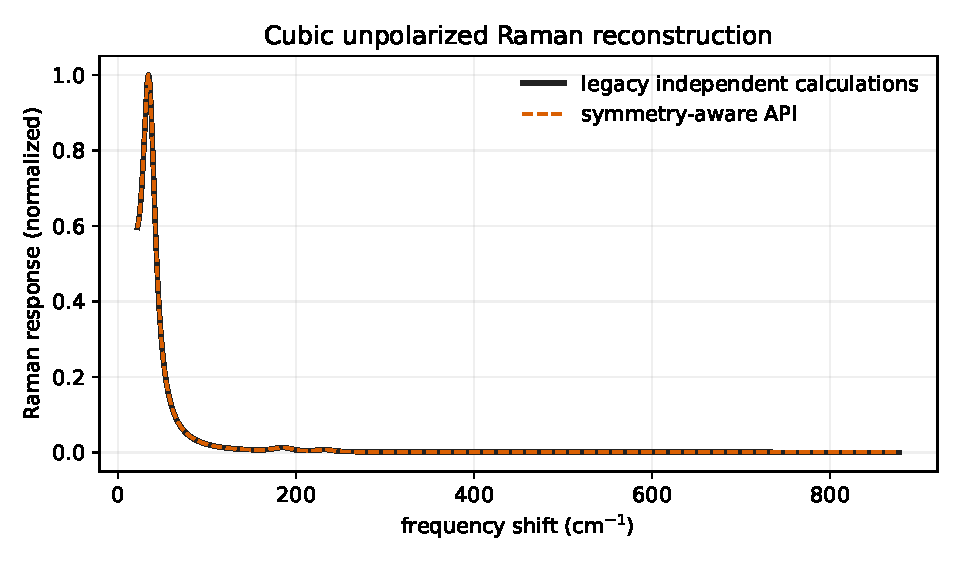
\includegraphics[width=0.84\linewidth]{figures/raman_legacy_vs_symmetry.pdf}
\caption{Controlled cubic unpolarized Raman response.  The legacy sum uses
three independent nonzero calculations; the new result reconstructs all
seven requested terms from one calculation and four exact zeros.  Curves are
visually coincident; the relative $L^\infty$ discrepancy is \RamanError.}
\label{fig:raman-spectrum}
\end{figure}

\begin{figure}[ht]
\centering
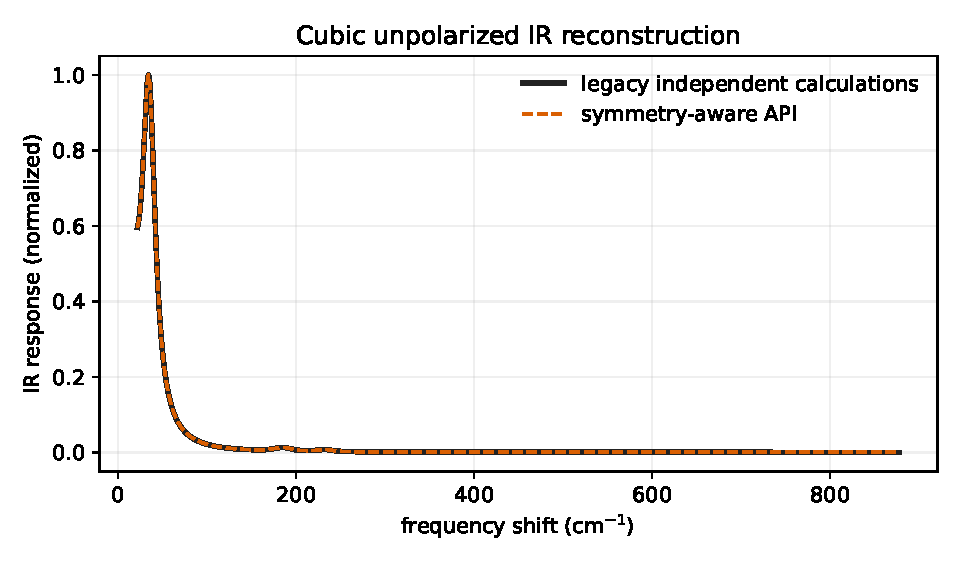
\includegraphics[width=0.84\linewidth]{figures/ir_legacy_vs_symmetry.pdf}
\caption{Controlled cubic unpolarized IR response.  Three legacy Cartesian
calculations are reconstructed from one symmetry representative.  The
relative $L^\infty$ discrepancy is \IRError.}
\label{fig:ir-spectrum}
\end{figure}

The agreement in \cref{fig:raman-spectrum,fig:ir-spectrum} is much tighter
than any physical statistical error in an SSCHA ensemble.  More importantly,
the test suite compares a single reduced application of the anharmonic
operator with the complete group average before Lanczos spectral analysis.
The real-space relative error is \RealKernelError{} and the q-space error is
\QKernelError{}.  This rules out the possibility that two visibly broadened
spectra merely hide different kernels.

\subsection{Additional correctness gates}

The focused suite exercises:
\begin{itemize}
  \item exact normalized/raw Raman invariant equivalence;
  \item polarized and coherent tensor contractions;
  \item real/q-space vertex and perturbation-modulus parity;
  \item cubic orbit reduction and anisotropic-mesh filtering;
  \item real/q-space full-average versus stabilizer/coset parity;
  \item direct q-space full-replica versus coset/inner-group parity on every
        point of a cubic $3\times3\times3$ mesh: $\Gamma$ and 26 non-TRI
        points, followed by a second application with a generated nonzero
        two-phonon input sector;
  \item atom-Fourier execution through inherited q-space preparation;
  \item directional atom-Fourier LO--TO basis pinning and interpolation-local
        effective-charge suppression that retains $Z^*$ for IR preparation;
  \item interrupted native restart, strict manifest mismatch rejection,
        portable \texttt{.abc} load, and load-only analysis;
  \item Bose detailed balance, Stokes minus anti-Stokes identity, and
        anisotropic tensorial IR electronic-background handling, including
        load-only inference and explicit override;
  \item zero symmetry-forbidden Raman channels; and
  \item uniform failure of every quarantined two-phonon/configuration-
        dependent optical entry point in base and derived classes.
\end{itemize}
At report generation time the focused spectroscopy/Raman/IR/interpolation
suite contains 69 passing
tests.  The complete non-heavy repository result is recorded in the project
handoff after the final audit run, so this document does not misstate a count
that changes when obsolete KPM tests are deleted.

\section{Performance analysis}
\label{sec:performance}

\begin{table}[ht]
\centering
\caption{End-to-end benchmark, including conservative new-workflow manifest
and checkpoint writes.  Times are wall seconds on the report-generation
host, not portable hardware constants.}
\label{tab:workflow-timing}
\begin{tabular}{@{}lrrr@{}}
\toprule
observable & legacy & new & speedup\\
\midrule
unpolarized Raman & \RamanLegacyTime & \RamanNewTime & \RamanSpeedup$\times$\\
unpolarized IR    & \IRLegacyTime    & \IRNewTime    & \IRSpeedup$\times$\\
\bottomrule
\end{tabular}
\end{table}

\begin{table}[ht]
\centering
\caption{Isolated anharmonic-operator benchmark at
\KernelConfigurations{} configurations.  Medians use seven repeated
applications after warm-up.}
\label{tab:kernel-timing}
\begin{tabular}{@{}lcccc@{}}
\toprule
backend & full $|G|$ & representatives & stabilizer $|H|$ & speedup\\
\midrule
real space & \GroupOrder & \CosetCount & \StabilizerOrder &
\RealKernelSpeedup$\times$\\
q space & \GroupOrder & \CosetCount & \StabilizerOrder &
\QKernelSpeedup$\times$\\
\bottomrule
\end{tabular}
\end{table}

\begin{figure}[ht]
\centering
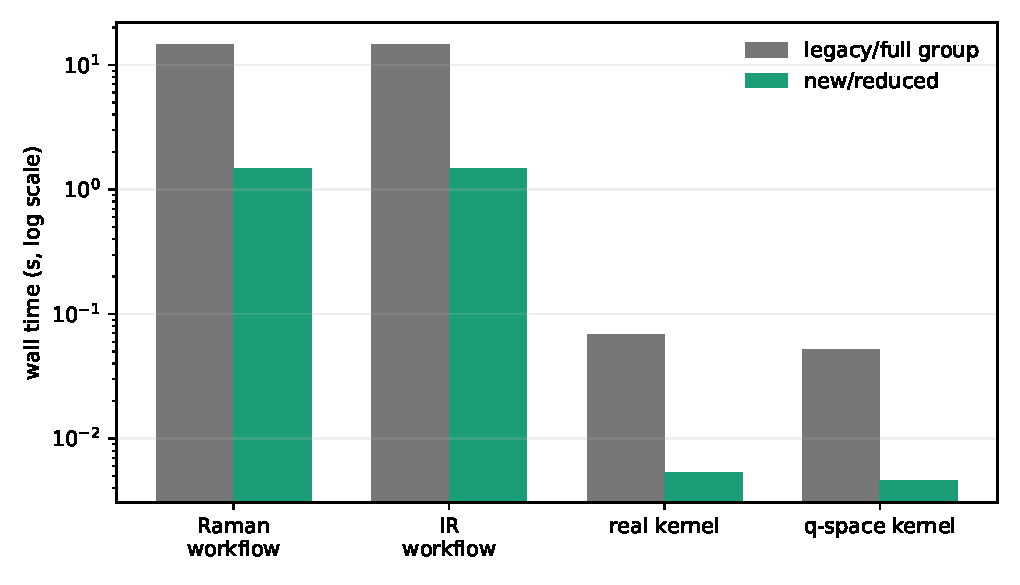
\includegraphics[width=0.86\linewidth]{figures/timings.pdf}
\caption{Measured workflow and isolated-kernel wall times.  The logarithmic
axis is necessary because a complete 256-step workflow and one kernel
application have different natural scales.}
\label{fig:timings}
\end{figure}

\begin{figure}[ht]
\centering
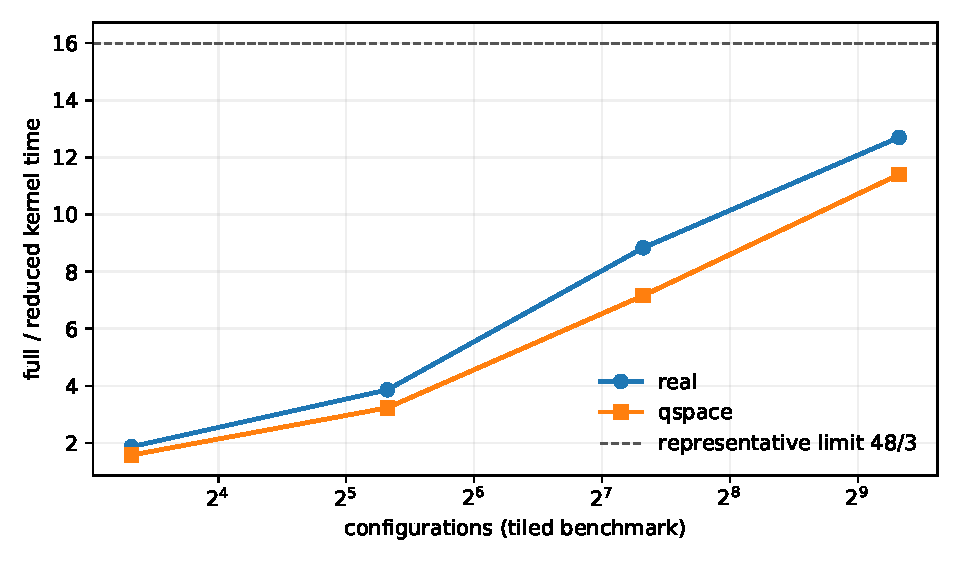
\includegraphics[width=0.82\linewidth]{figures/kernel_scaling.pdf}
\caption{Measured kernel speedup after deterministically tiling the same ten
configurations.  Tiling leaves the normalized ensemble average unchanged and
isolates computational scaling; it does not claim improved statistical
sampling.  The dashed line is the asymptotic representative ratio $48/3=16$.}
\label{fig:kernel-scaling}
\end{figure}

Three effects contribute to the workflow improvement:
\begin{enumerate}
  \item \textbf{Across observables:} three equivalent Raman or IR channels are
        represented by one run.
  \item \textbf{Translations:} a $\Gamma$ optical perturbation separates the
        cheap translation projector from the expensive point-group ensemble
        replication.  The direct legacy real-space path used the full
        supercell space-group list.
  \item \textbf{Within one run:} \GroupOrder{} point-group operations reduce
        to \CosetCount{} expensive representatives, followed by the
        \StabilizerOrder-term linear-algebra projector.
\end{enumerate}
These factors are not expected to multiply into an exact wall-time ratio:
initialization, Python/Julia calls, BLAS work, checkpoint I/O, and the
stabilizer projector remain.  In particular, the projector is independent of
the number of configurations and performs \StabilizerOrder{} sparse
vector/rank-two transformations after the representative average.  With only
ten configurations that fixed work is comparable to evaluating three
representatives, giving the initially puzzling 1.87$\times$ (real) and
1.58$\times$ (q-space) speedups.  At 40, 160, and 640 configurations the
measured real-space ratios are 3.86, 8.83, and
\RealKernelSpeedup; q-space gives 3.23, 7.16, and
\QKernelSpeedup.  This monotone approach toward $48/3=16$ verifies that the
optimization scales as predicted rather than hiding a replicated-ensemble
calculation in the projector.  The isolated-kernel speedups in
\cref{tab:kernel-timing} are therefore the clean measure of the new coset
optimization, while \cref{tab:workflow-timing} measures what a legacy script
and a restartable production workflow actually experienced on this fixture.

A six-step microbenchmark was also inspected during the audit.  There, atomic
checkpoint and manifest writes dominated and made the new workflow slower
than three unsaved legacy calls even though its kernel was faster.  This is
expected fixed-cost behavior, not a hidden regression.  The reported
\BenchSteps-step case is still small but makes recurrence work visible.

\section{Code audit and removal decisions}
\label{sec:audit}

\subsection{Findings corrected in this branch}

\begin{longtable}{@{}p{0.22\linewidth}p{0.69\linewidth}@{}}
\toprule
area & audit result\\
\midrule
\endhead
Raman definitions & One canonical component table now generates both legacy
normalizations and the new API.  The former channel-accumulation overwrite
cannot recur in a second copy.\\[3pt]
Derived classes & QSpaceLanczos and QSpaceAtomFourier do not duplicate public
Raman/IR preparation.  Only representation-specific $\Gamma$ preparation and
operator application remain overridden.\\[3pt]
Finite q & The q-space backend now retains its exact sparse Bloch
representation and detects finite-q little groups with complex characters.
Full/coset parity is checked for all 27 points of an odd cubic mesh and for a
nonzero two-phonon input.\\[3pt]
Zero channels & Exactly zero Raman derivatives are valid symmetry-forbidden
contributions.  The planner now records them with no run identifier, and the
evaluator skips them as mathematical zeros.\\[3pt]
Scale independence & Symmetry matching and canonical signs use relative
vector tolerances.  Roundoff-level forbidden components are detected relative
to the strongest channel in the same request, so a physically small but
nonzero optical tensor is not quantized away.\\[3pt]
Global deduplication & Orbit analysis is performed over all named requests at
once.  Separately added cubic \texttt{ir\_x} and \texttt{ir\_y} requests now
share one run while retaining independent reconstruction weights.\\[3pt]
Group order & Unit-cell crystallographic rotations are matched to the
backend's native ordering by matrix comparison.  The code does not assume
spglib and CellConstructor enumerate operations identically.\\[3pt]
Coset side & Right cosets are used consistently with the representation action
and checked through full-average parity tests.\\[3pt]
Rank-two output & The stabilizer is applied to both force and second-derivative
terms, including every q-space momentum-pair block.\\[3pt]
Restart writes & Native status uses a temporary filename that preserves the
\texttt{.npz} extension before atomic replacement; interruption/resume is
tested.\\[3pt]
IR units & The raw Rydberg Green function receives the explicit factor two for
Hartree susceptibility.  $4\pi/\Omega$ uses bohr$^3$, and the electronic
dielectric projection uses the full tensor, inferred from the dynamical
matrix or stored manifest unless explicitly overridden.\\[3pt]
Backend switches & \texttt{ignore\_v3}, \texttt{ignore\_v4}, and
\texttt{lo\_to\_split} are public, manifest-recorded options; legacy
\texttt{backend\_options} scripts remain accepted.  Atom-Fourier implements
directional LO--TO interpolation rather than raising
\texttt{NotImplementedError}.\\[3pt]
KPM & Backend module, build/install entry, CLI/script loaders, documentation,
and KPM tests were purged.  Repository-wide textual audit finds no KPM API
reference.  Git history remains the recovery mechanism.\\[3pt]
Two-phonon optics & Public legacy names remain only to fail loudly with
\texttt{NotImplementedError}.  The Raman source backup is private, unimported,
and excluded from installation.\\
\bottomrule
\end{longtable}

\subsection{Deliberate limitations}

The following are not silently approximated:
\begin{itemize}
  \item configuration-dependent/two-phonon Raman and IR vertices;
  \item resonant or antisymmetric Raman tensors;
  \item cross-correlations between two distinct external vertices;
  \item absolute experimental Raman cross sections;
  \item automatic SI absorption or conductivity conversions; and
  \item interpreting the controlled benchmark as a material prediction.
\end{itemize}
The stable API covers equilibrium one-phonon polarized/unpolarized Raman and
IR response.  Adding any item above should begin from a written observable
definition and symmetry transformation law, then acquire full-average parity
tests before being exposed.

\section{Reproducibility}

From the repository root, regenerate numerical data and vector figures with
\begin{lstlisting}[language=bash]
micromamba run -n sscha \
  python spectroscopy_report/benchmark_spectroscopy.py
\end{lstlisting}
The script writes
\texttt{data/benchmark\_summary.json},
\texttt{data/spectra.csv}, generated \LaTeX{} macros, and the four PDF
figures.  Compile this report from its own directory:
\begin{lstlisting}[language=bash]
lualatex -interaction=nonstopmode -halt-on-error \
  tdscha_spectroscopy_report.tex
lualatex -interaction=nonstopmode -halt-on-error \
  tdscha_spectroscopy_report.tex
\end{lstlisting}
This directory is intentionally independent of
\texttt{report/interpolation/}.  Neither its source, figures, data, nor PDF is
shared with the interpolation report.

\section{Conclusions}

The refactor makes the default behavior unambiguous: users name a polarized
or unpolarized Raman/IR observable, inspect a symmetry plan, and run it through
one restartable driver.  Legacy equilibrium calls continue to work, but no
longer define physics independently.  The two formerly competing
unpolarized Raman routines are recognized as equivalent normalizations; the
historically broken normalized implementation is repaired through shared
construction and regression tests.

The group-theory optimization is exact linear algebra.  Orbits remove
equivalent requested experiments; stabilizers and right cosets rearrange the
same ensemble average inside each application of $\mathcal L$.  Both levels
are verified against unreduced calculations.  The cubic test reconstructs
Raman and IR spectra at $10^{-14}$ relative accuracy with one independent run
per observable, and the measured timing improvement is substantial once the
recurrence exceeds fixed checkpoint overhead.

The resulting code has one optical-definition layer, one workflow layer, and
small backend adapters.  Obsolete KPM code is gone and unvalidated two-phonon
code cannot be invoked accidentally.  This provides a clean base on which
future optical vertices can be added only after their physics and symmetry
are independently validated.

\appendix
\section{Algebraic equivalence of Raman normalizations}

Let a raw component be $\bm v$ with response
$\mathcal R_{\bm v}$.  Because a diagonal linear response is bilinear in its
two external vertices,
\begin{equation}
  \mathcal R_{s\bm v}=s^2\mathcal R_{\bm v}.
\end{equation}
For the isotropic component $s=1/3$, so
\begin{equation}
  45\mathcal R_{\bm v/3}=45\frac{1}{9}\mathcal R_{\bm v}
  =5\mathcal R_{\bm v}.
\end{equation}
For a diagonal deviator $s=1/\sqrt2$,
$7s^2=7/2$.  For an off-diagonal component $s=\sqrt3$,
$7s^2=21$.  This proves every row of
\cref{tab:legacy-normalizations}; it also explains why saved spectra cannot be
combined safely unless their component convention is known.

\section{Why a zero component needs no Lanczos run}

If $\bm v=\bm0$, then the external coupling in
\cref{eq:external-coupling} vanishes.  Bilinearity gives
\begin{equation}
  G_{0,0}(\omega)=0,
  \qquad \mathcal R_0(\omega)=0.
\end{equation}
Attempting Lanczos recursion would require normalizing the zero initial vector
and is undefined.  Therefore ``record zero, schedule nothing'' is both the
mathematically correct behavior and the numerically safe behavior.

\section{Manifest interpretation of symmetry reconstruction}

For each requested component the manifest stores
\begin{equation}
  (\texttt{run\_id},w_j,\chi_j,j).
\end{equation}
A null \texttt{run\_id} means the component is identically zero.  Otherwise
all components with the same identifier share one cached diagonal Green
function.  Because $G_{-v,-v}=G_{v,v}$, $\chi_j$ is not multiplied into a
diagonal intensity.  It remains essential metadata for any future
$G_{v_i,v_j}$ cross response, where the relative sign does matter.

\begin{thebibliography}{9}

\bibitem{monacelli2021}
L.~Monacelli and F.~Mauri,
``Time-dependent self-consistent harmonic approximation: Anharmonic nuclear
quantum dynamics and time correlation functions,''
\emph{Physical Review B} \textbf{103}, 104305 (2021),
\href{https://doi.org/10.1103/PhysRevB.103.104305}{doi:10.1103/PhysRevB.103.104305}.

\bibitem{siciliano2023}
A.~Siciliano, L.~Monacelli, G.~Caldarelli, and F.~Mauri,
``Wigner Gaussian dynamics: Simulating the anharmonic and quantum ionic
motion,'' \emph{Physical Review B} \textbf{107}, 174307 (2023),
\href{https://doi.org/10.1103/PhysRevB.107.174307}{doi:10.1103/PhysRevB.107.174307}.

\bibitem{lanczos1950}
C.~Lanczos, ``An iteration method for the solution of the eigenvalue problem
of linear differential and integral operators,''
\emph{Journal of Research of the National Bureau of Standards}
\textbf{45}, 255--282 (1950).

\bibitem{placzek1934}
G.~Placzek, ``Rayleigh-Streuung und Raman-Effekt,'' in
\emph{Handbuch der Radiologie}, Vol.~VI, Part~II (Akademische
Verlagsgesellschaft, Leipzig, 1934), pp.~205--374.

\bibitem{popov2020}
M.~N. Popov, J.~Spitaler, V.~K. Veerapandiyan, E.~Bousquet, J.~Hlinka, and
M.~Deluca, ``Raman spectra of fine-grained materials from first principles,''
\emph{npj Computational Materials} \textbf{6}, 121 (2020),
\href{https://doi.org/10.1038/s41524-020-00395-3}{doi:10.1038/s41524-020-00395-3}.

\bibitem{togo2024}
A.~Togo, K.~Shinohara, and I.~Tanaka,
``Spglib: a software library for crystal symmetry search,''
\emph{Science and Technology of Advanced Materials: Methods}
\textbf{4}, 2384822 (2024),
\href{https://doi.org/10.1080/27660400.2024.2384822}{doi:10.1080/27660400.2024.2384822}.

\end{thebibliography}

\end{document}
